\documentclass[a4paper]{book}
\usepackage{a4wide}
\usepackage{makeidx}
\usepackage{graphicx}
\usepackage{multicol}
\usepackage{float}
\usepackage{listings}
\usepackage{color}
\usepackage{textcomp}
\usepackage{alltt}
\usepackage{times}
\usepackage{ifpdf}
\ifpdf
\usepackage[pdftex,
            pagebackref=true,
            colorlinks=true,
            linkcolor=blue,
            unicode
           ]{hyperref}
\else
\usepackage[ps2pdf,
            pagebackref=true,
            colorlinks=true,
            linkcolor=blue,
            unicode
           ]{hyperref}
\usepackage{pspicture}
\fi
\usepackage[utf8]{inputenc}
\usepackage{doxygen}
\lstset{language=C++,inputencoding=utf8,basicstyle=\footnotesize,breaklines=true,breakatwhitespace=true,tabsize=8,numbers=left }
\makeindex
\setcounter{tocdepth}{3}
\renewcommand{\footrulewidth}{0.4pt}
\begin{document}
\hypersetup{pageanchor=false}
\begin{titlepage}
\vspace*{7cm}
\begin{center}
{\Large Reference Manual}\\
\vspace*{1cm}
{\large Generated by Doxygen 1.7.1}\\
\vspace*{0.5cm}
{\small Tue Mar 29 2011 21:40:55}\\
\end{center}
\end{titlepage}
\clearemptydoublepage
\pagenumbering{roman}
\tableofcontents
\clearemptydoublepage
\pagenumbering{arabic}
\hypersetup{pageanchor=true}
\chapter{Class Index}
\section{Class List}
Here are the classes, structs, unions and interfaces with brief descriptions:\begin{DoxyCompactList}
\item\contentsline{section}{\hyperlink{classControl}{Control} }{\pageref{classControl}}{}
\item\contentsline{section}{\hyperlink{classCSE}{CSE} }{\pageref{classCSE}}{}
\item\contentsline{section}{\hyperlink{classEnvironment}{Environment} }{\pageref{classEnvironment}}{}
\item\contentsline{section}{\hyperlink{classRpal}{Rpal} }{\pageref{classRpal}}{}
\item\contentsline{section}{\hyperlink{classRpalError}{RpalError} }{\pageref{classRpalError}}{}
\item\contentsline{section}{\hyperlink{classRpalLexer}{RpalLexer} }{\pageref{classRpalLexer}}{}
\item\contentsline{section}{\hyperlink{classRpalParser}{RpalParser} }{\pageref{classRpalParser}}{}
\item\contentsline{section}{\hyperlink{classStandardizer}{Standardizer} }{\pageref{classStandardizer}}{}
\item\contentsline{section}{\hyperlink{classToken}{Token} }{\pageref{classToken}}{}
\item\contentsline{section}{\hyperlink{classTreeNode}{TreeNode} }{\pageref{classTreeNode}}{}
\end{DoxyCompactList}

\chapter{Class Documentation}
\hypertarget{classControl}{
\section{Control Class Reference}
\label{classControl}\index{Control@{Control}}
}


Collaboration diagram for Control:\nopagebreak
\begin{figure}[H]
\begin{center}
\leavevmode
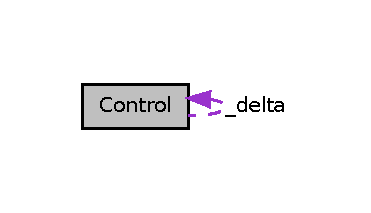
\includegraphics[width=178pt]{classControl__coll__graph}
\end{center}
\end{figure}
\subsection*{Public Types}
\begin{DoxyCompactItemize}
\item 
enum {\bfseries Type} \{ \par
{\bfseries ENV} =  1, 
{\bfseries DELTA} =  2, 
{\bfseries NAME} =  3, 
{\bfseries LAMBDA} =  4, 
\par
{\bfseries GAMMA} =  5, 
{\bfseries AUG} =  6, 
{\bfseries BETA} =  7, 
{\bfseries OR} =  8, 
\par
{\bfseries AND\_\-LOGICAL} =  9, 
{\bfseries NOT} =  10, 
{\bfseries GR} =  11, 
{\bfseries GE} =  12, 
\par
{\bfseries LS} =  13, 
{\bfseries LE} =  14, 
{\bfseries EQ} =  15, 
{\bfseries NE} =  16, 
\par
{\bfseries ADD} =  17, 
{\bfseries SUBTRACT} =  18, 
{\bfseries NEG} =  19, 
{\bfseries MULTIPLY} =  20, 
\par
{\bfseries DIVIDE} =  21, 
{\bfseries EXP} =  22, 
{\bfseries AT} =  23, 
{\bfseries TRUE} =  24, 
\par
{\bfseries FALSE} =  25, 
{\bfseries NIL} =  26, 
{\bfseries DUMMY} =  27, 
{\bfseries YSTAR} =  28, 
\par
{\bfseries ETA} =  29, 
{\bfseries TAU} =  30, 
{\bfseries STRING} =  31, 
{\bfseries INTEGER} =  32, 
\par
{\bfseries TUPLE} =  33
 \}
\end{DoxyCompactItemize}
\subsection*{Public Member Functions}
\begin{DoxyCompactItemize}
\item 
\hypertarget{classControl_a3bebd50d64be06d324f460bd6bb3289e}{
void {\bfseries add\_\-control} (\hyperlink{classTreeNode}{TreeNode} $\ast$node, int, string, vector$<$ string $>$ $\ast$, \hyperlink{classControl}{Control} $\ast$, int)}
\label{classControl_a3bebd50d64be06d324f460bd6bb3289e}

\item 
\hypertarget{classControl_a253c2963cf1561f52e3212a2a91dd09a}{
void {\bfseries pretty\_\-print} ()}
\label{classControl_a253c2963cf1561f52e3212a2a91dd09a}

\item 
\hypertarget{classControl_a4c41c3158d8913e39e10f207d59592ff}{
string {\bfseries to\_\-s} ()}
\label{classControl_a4c41c3158d8913e39e10f207d59592ff}

\item 
\hypertarget{classControl_a578b3b8a92a99a8924bbaaa35765caa6}{
{\bfseries Control} (\hyperlink{classControl}{Control} $\ast$cntrl)}
\label{classControl_a578b3b8a92a99a8924bbaaa35765caa6}

\item 
\hypertarget{classControl_aed0474eda3fbba2470cfdd5865cdf95e}{
{\bfseries Control} (Control::Type type, int index)}
\label{classControl_aed0474eda3fbba2470cfdd5865cdf95e}

\item 
\hypertarget{classControl_a6f035fbbd272ba6a877554cb9c46846b}{
{\bfseries Control} (Control::Type type, vector$<$ string $>$ $\ast$variables, \hyperlink{classControl}{Control} $\ast$del\_\-ptr, int delta\_\-index)}
\label{classControl_a6f035fbbd272ba6a877554cb9c46846b}

\item 
\hypertarget{classControl_ac37be7f2ad830c2a56337ae86e8a8e4e}{
{\bfseries Control} (Control::Type type, int index, bool watever)}
\label{classControl_ac37be7f2ad830c2a56337ae86e8a8e4e}

\item 
\hypertarget{classControl_af4d697c95ee5886169013e12ef016f34}{
{\bfseries Control} (string var\_\-value, Control::Type type)}
\label{classControl_af4d697c95ee5886169013e12ef016f34}

\item 
\hypertarget{classControl_a2b72ec8881d3e7261feb61999b5ea8f2}{
{\bfseries Control} (Control::Type type, string value)}
\label{classControl_a2b72ec8881d3e7261feb61999b5ea8f2}

\item 
\hypertarget{classControl_ad6aff5424c3c8757ff944e82811bd263}{
{\bfseries Control} (Control::Type type)}
\label{classControl_ad6aff5424c3c8757ff944e82811bd263}

\item 
\hypertarget{classControl_a29657151fef124d4d312f0b7802d8456}{
Type {\bfseries type} ()}
\label{classControl_a29657151fef124d4d312f0b7802d8456}

\item 
\hypertarget{classControl_a211f56b0c94aae1ada32afff1c0b1988}{
string {\bfseries value} ()}
\label{classControl_a211f56b0c94aae1ada32afff1c0b1988}

\item 
\hypertarget{classControl_a9421d4639d1f2d15c512611f762db55b}{
int {\bfseries index} ()}
\label{classControl_a9421d4639d1f2d15c512611f762db55b}

\item 
\hypertarget{classControl_a68fb29afe121b4b000bbac2d4dfe7040}{
void {\bfseries set\_\-linked\_\-env\_\-id} (int id)}
\label{classControl_a68fb29afe121b4b000bbac2d4dfe7040}

\item 
\hypertarget{classControl_a9e04b57a5854cb28af2318f59ec12fe4}{
int {\bfseries linked\_\-env\_\-id} ()}
\label{classControl_a9e04b57a5854cb28af2318f59ec12fe4}

\item 
\hypertarget{classControl_a96b36fd85014457b43388b84dd125878}{
void {\bfseries set\_\-type} (Type type)}
\label{classControl_a96b36fd85014457b43388b84dd125878}

\item 
\hypertarget{classControl_a36e7d957ed52b30ace86d16315004284}{
void {\bfseries set\_\-value} (string value)}
\label{classControl_a36e7d957ed52b30ace86d16315004284}

\end{DoxyCompactItemize}
\subsection*{Public Attributes}
\begin{DoxyCompactItemize}
\item 
\hypertarget{classControl_a789fac1709329ea69d67ab52f9be7ca7}{
vector$<$ \hyperlink{classControl}{Control} $\ast$ $>$ $\ast$ {\bfseries \_\-control\_\-struct}}
\label{classControl_a789fac1709329ea69d67ab52f9be7ca7}

\item 
\hypertarget{classControl_afc67e4eb74a62032e271646d3b91ebf9}{
vector$<$ string $>$ {\bfseries \_\-variables}}
\label{classControl_afc67e4eb74a62032e271646d3b91ebf9}

\item 
\hypertarget{classControl_ad761965741b7aef5f3918d4815e9b4cb}{
vector$<$ \hyperlink{classControl}{Control} $\ast$ $>$ {\bfseries \_\-tuples}}
\label{classControl_ad761965741b7aef5f3918d4815e9b4cb}

\end{DoxyCompactItemize}


The documentation for this class was generated from the following files:\begin{DoxyCompactItemize}
\item 
control.h\item 
control.c++\end{DoxyCompactItemize}

\hypertarget{classCSE}{
\section{CSE Class Reference}
\label{classCSE}\index{CSE@{CSE}}
}


Collaboration diagram for CSE:\nopagebreak
\begin{figure}[H]
\begin{center}
\leavevmode
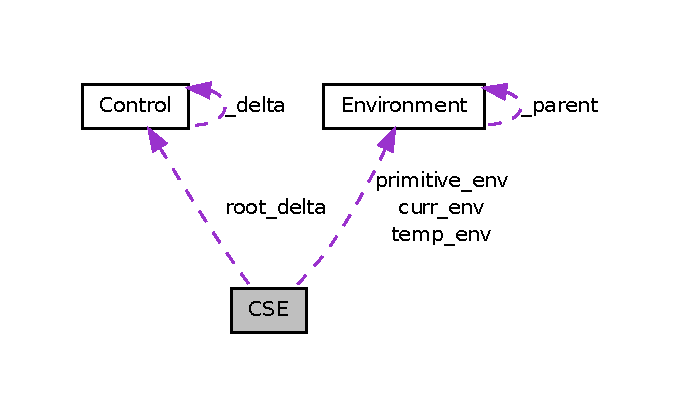
\includegraphics[width=327pt]{classCSE__coll__graph}
\end{center}
\end{figure}
\subsection*{Public Member Functions}
\begin{DoxyCompactItemize}
\item 
\hypertarget{classCSE_a9c228b4b996b105db362bf06b909b242}{
void {\bfseries run} (\hyperlink{classTreeNode}{TreeNode} $\ast$root)}
\label{classCSE_a9c228b4b996b105db362bf06b909b242}

\end{DoxyCompactItemize}


The documentation for this class was generated from the following file:\begin{DoxyCompactItemize}
\item 
cse.c++\end{DoxyCompactItemize}

\hypertarget{classEnvironment}{
\section{Environment Class Reference}
\label{classEnvironment}\index{Environment@{Environment}}
}


Collaboration diagram for Environment:\nopagebreak
\begin{figure}[H]
\begin{center}
\leavevmode
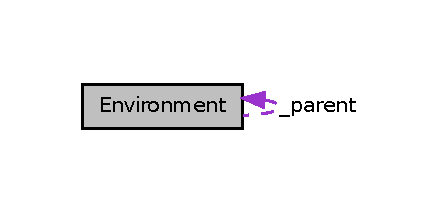
\includegraphics[width=211pt]{classEnvironment__coll__graph}
\end{center}
\end{figure}
\subsection*{Public Member Functions}
\begin{DoxyCompactItemize}
\item 
\hypertarget{classEnvironment_a6222137be37777f9a9b101cd0f4742ec}{
void {\bfseries assign\_\-parent} (\hyperlink{classEnvironment}{Environment} $\ast$parent)}
\label{classEnvironment_a6222137be37777f9a9b101cd0f4742ec}

\item 
\hypertarget{classEnvironment_a340ef027cc02e3f17859f236086a1bfd}{
\hyperlink{classControl}{Control} $\ast$ {\bfseries lookup} (string symbol)}
\label{classEnvironment_a340ef027cc02e3f17859f236086a1bfd}

\item 
\hypertarget{classEnvironment_a870868346d63e873806b347e0b6619b9}{
{\bfseries Environment} (int id)}
\label{classEnvironment_a870868346d63e873806b347e0b6619b9}

\item 
\hypertarget{classEnvironment_a38a3ee60ad7bc5f4e8829a5f6b301000}{
int {\bfseries id} () const }
\label{classEnvironment_a38a3ee60ad7bc5f4e8829a5f6b301000}

\item 
\hypertarget{classEnvironment_a4e5d19483e7d71196b8a798f18e4146d}{
void {\bfseries pretty\_\-print} ()}
\label{classEnvironment_a4e5d19483e7d71196b8a798f18e4146d}

\end{DoxyCompactItemize}
\subsection*{Public Attributes}
\begin{DoxyCompactItemize}
\item 
\hypertarget{classEnvironment_ae86ce99694878510782a516082bdad0f}{
map$<$ string, \hyperlink{classControl}{Control} $\ast$ $>$ {\bfseries symbol\_\-table}}
\label{classEnvironment_ae86ce99694878510782a516082bdad0f}

\end{DoxyCompactItemize}


The documentation for this class was generated from the following file:\begin{DoxyCompactItemize}
\item 
environment.c++\end{DoxyCompactItemize}

\hypertarget{classRpal}{
\section{Rpal Class Reference}
\label{classRpal}\index{Rpal@{Rpal}}
}


Collaboration diagram for Rpal:\nopagebreak
\begin{figure}[H]
\begin{center}
\leavevmode
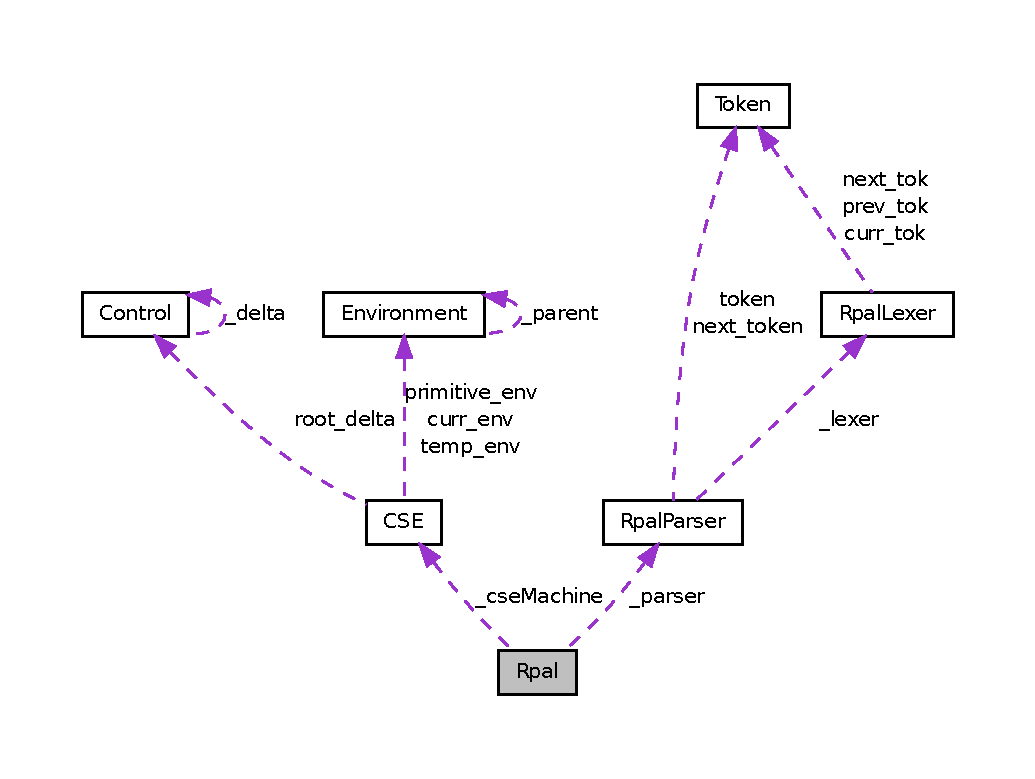
\includegraphics[width=400pt]{classRpal__coll__graph}
\end{center}
\end{figure}
\subsection*{Public Member Functions}
\begin{DoxyCompactItemize}
\item 
\hypertarget{classRpal_a974dfca706a0b14239c882a9205f2042}{
{\bfseries Rpal} (\hyperlink{classRpalParser}{RpalParser} $\ast$parser)}
\label{classRpal_a974dfca706a0b14239c882a9205f2042}

\item 
\hypertarget{classRpal_a0ffb4c66518df139fb848906b13dac0d}{
void {\bfseries printAST} ()}
\label{classRpal_a0ffb4c66518df139fb848906b13dac0d}

\item 
\hypertarget{classRpal_acb2e83e6257ad29b56c4c1927ce24c1a}{
void {\bfseries printST} ()}
\label{classRpal_acb2e83e6257ad29b56c4c1927ce24c1a}

\item 
\hypertarget{classRpal_ab04297169437ac8825c424f5c90e2fc8}{
void {\bfseries execute} ()}
\label{classRpal_ab04297169437ac8825c424f5c90e2fc8}

\end{DoxyCompactItemize}


The documentation for this class was generated from the following file:\begin{DoxyCompactItemize}
\item 
rpal.c++\end{DoxyCompactItemize}

\hypertarget{classRpalError}{
\section{RpalError Class Reference}
\label{classRpalError}\index{RpalError@{RpalError}}
}
\subsection*{Public Member Functions}
\begin{DoxyCompactItemize}
\item 
\hypertarget{classRpalError_ac9862399f06a5e9001ee663749b5bbe4}{
{\bfseries RpalError} (int type, string message)}
\label{classRpalError_ac9862399f06a5e9001ee663749b5bbe4}

\item 
\hypertarget{classRpalError_aa7fff0f806c4457e51e9ae2d0204038e}{
virtual const char $\ast$ {\bfseries what} () const   throw ()}
\label{classRpalError_aa7fff0f806c4457e51e9ae2d0204038e}

\end{DoxyCompactItemize}
\subsection*{Static Public Attributes}
\begin{DoxyCompactItemize}
\item 
\hypertarget{classRpalError_a1f24d53b71e810c422d690586fa191b1}{
static const int {\bfseries LEXER} = 1}
\label{classRpalError_a1f24d53b71e810c422d690586fa191b1}

\item 
\hypertarget{classRpalError_ac3b5a0c5e6c03d56a84fa2b710ac8cfe}{
static const int {\bfseries PARSER} = 2}
\label{classRpalError_ac3b5a0c5e6c03d56a84fa2b710ac8cfe}

\item 
\hypertarget{classRpalError_af7451154cdf3f52dac9cc5c5dfc3e852}{
static const int {\bfseries INTERNAL} = 3}
\label{classRpalError_af7451154cdf3f52dac9cc5c5dfc3e852}

\item 
\hypertarget{classRpalError_a37990c79901770f8e6482721bef99ab6}{
static const int {\bfseries INTERPRETER} = 4}
\label{classRpalError_a37990c79901770f8e6482721bef99ab6}

\end{DoxyCompactItemize}


The documentation for this class was generated from the following file:\begin{DoxyCompactItemize}
\item 
rpalerror.h\end{DoxyCompactItemize}

\hypertarget{classRpalLexer}{
\section{RpalLexer Class Reference}
\label{classRpalLexer}\index{RpalLexer@{RpalLexer}}
}


Collaboration diagram for RpalLexer:\nopagebreak
\begin{figure}[H]
\begin{center}
\leavevmode
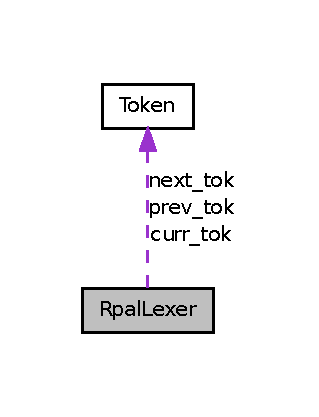
\includegraphics[width=153pt]{classRpalLexer__coll__graph}
\end{center}
\end{figure}
\subsection*{Public Member Functions}
\begin{DoxyCompactItemize}
\item 
\hypertarget{classRpalLexer_a60edfae72ab9992fbff1f4867cb8614b}{
{\bfseries RpalLexer} (ifstream $\ast$fileHandle)}
\label{classRpalLexer_a60edfae72ab9992fbff1f4867cb8614b}

\item 
\hypertarget{classRpalLexer_af97ac9808131f59c9eadff33cd8fdcc3}{
const \hyperlink{classToken}{Token} $\ast$ {\bfseries nextToken} ()}
\label{classRpalLexer_af97ac9808131f59c9eadff33cd8fdcc3}

\end{DoxyCompactItemize}


The documentation for this class was generated from the following files:\begin{DoxyCompactItemize}
\item 
lexer.h\item 
lexer.c++\end{DoxyCompactItemize}

\hypertarget{classRpalParser}{
\section{RpalParser Class Reference}
\label{classRpalParser}\index{RpalParser@{RpalParser}}
}


Collaboration diagram for RpalParser:\nopagebreak
\begin{figure}[H]
\begin{center}
\leavevmode
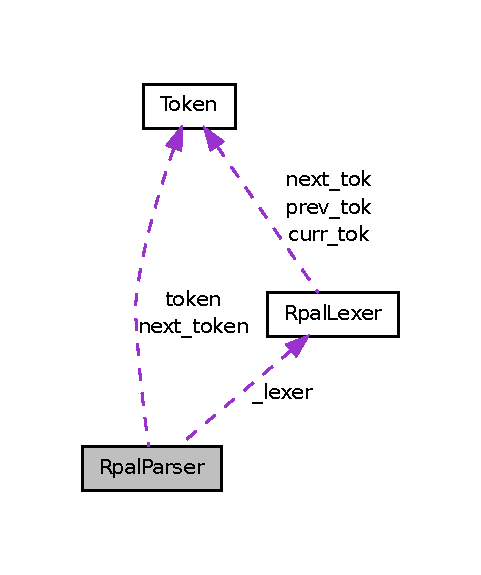
\includegraphics[width=231pt]{classRpalParser__coll__graph}
\end{center}
\end{figure}
\subsection*{Public Member Functions}
\begin{DoxyCompactItemize}
\item 
\hypertarget{classRpalParser_a2252a6696fd900cee1acf1fb76bff546}{
stack$<$ \hyperlink{classTreeNode}{TreeNode} $\ast$ $>$ $\ast$ {\bfseries parse} ()}
\label{classRpalParser_a2252a6696fd900cee1acf1fb76bff546}

\item 
\hypertarget{classRpalParser_af1bf1d4d566c5011129f3bfe0aa4feb3}{
{\bfseries RpalParser} (\hyperlink{classRpalLexer}{RpalLexer} $\ast$lexer)}
\label{classRpalParser_af1bf1d4d566c5011129f3bfe0aa4feb3}

\end{DoxyCompactItemize}


The documentation for this class was generated from the following files:\begin{DoxyCompactItemize}
\item 
parser.h\item 
parser.c++\end{DoxyCompactItemize}

\hypertarget{classStandardizer}{
\section{Standardizer Class Reference}
\label{classStandardizer}\index{Standardizer@{Standardizer}}
}
\subsection*{Public Member Functions}
\begin{DoxyCompactItemize}
\item 
\hypertarget{classStandardizer_a77273774dcf6da7cef36af92d7ea7a3c}{
void {\bfseries standerdize} (\hyperlink{classTreeNode}{TreeNode} $\ast$ast\_\-tree)}
\label{classStandardizer_a77273774dcf6da7cef36af92d7ea7a3c}

\end{DoxyCompactItemize}


The documentation for this class was generated from the following file:\begin{DoxyCompactItemize}
\item 
standardizer.c++\end{DoxyCompactItemize}

\hypertarget{classToken}{
\section{Token Class Reference}
\label{classToken}\index{Token@{Token}}
}
\subsection*{Public Types}
\begin{DoxyCompactItemize}
\item 
enum {\bfseries Types} \{ \par
{\bfseries IDENTIFIER} =  0, 
{\bfseries INTEGER} =  1, 
{\bfseries OPERATOR} =  2, 
{\bfseries STRING} =  3, 
\par
{\bfseries DELETE} =  4, 
{\bfseries PUNCTION} =  5, 
{\bfseries ENDOFFILE} =  6
 \}
\end{DoxyCompactItemize}
\subsection*{Public Member Functions}
\begin{DoxyCompactItemize}
\item 
\hypertarget{classToken_aecbb17ed64896506113b557b3fb0e497}{
{\bfseries Token} (string token\_\-value)}
\label{classToken_aecbb17ed64896506113b557b3fb0e497}

\item 
\hypertarget{classToken_a2d65336967e81971f5d59b3ef23bd264}{
{\bfseries Token} (int type\_\-of\_\-tok)}
\label{classToken_a2d65336967e81971f5d59b3ef23bd264}

\item 
\hypertarget{classToken_aba1d7c5066f3ce760f6a6b6526b09618}{
{\bfseries Token} (int type\_\-of\_\-tok, string token\_\-value)}
\label{classToken_aba1d7c5066f3ce760f6a6b6526b09618}

\item 
\hypertarget{classToken_a09c0ff9720be0b1f7592630aaea902c2}{
int {\bfseries type} () const }
\label{classToken_a09c0ff9720be0b1f7592630aaea902c2}

\item 
\hypertarget{classToken_aae6417b57687404d09cdf35a3e2efa28}{
string {\bfseries value} () const }
\label{classToken_aae6417b57687404d09cdf35a3e2efa28}

\item 
\hypertarget{classToken_af8e3abaeea6dc77de44265d5d1d52438}{
string {\bfseries to\_\-s} () const }
\label{classToken_af8e3abaeea6dc77de44265d5d1d52438}

\end{DoxyCompactItemize}


The documentation for this class was generated from the following file:\begin{DoxyCompactItemize}
\item 
token.c++\end{DoxyCompactItemize}

\hypertarget{classTreeNode}{
\section{TreeNode Class Reference}
\label{classTreeNode}\index{TreeNode@{TreeNode}}
}


Collaboration diagram for TreeNode:\nopagebreak
\begin{figure}[H]
\begin{center}
\leavevmode
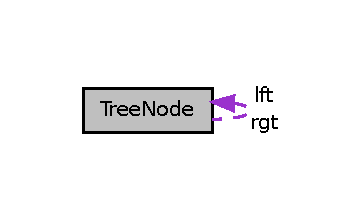
\includegraphics[width=174pt]{classTreeNode__coll__graph}
\end{center}
\end{figure}
\subsection*{Public Types}
\begin{DoxyCompactItemize}
\item 
enum {\bfseries Type} \{ \par
{\bfseries LAMBDA} =  1, 
{\bfseries WHERE} =  2, 
{\bfseries TAU} =  3, 
{\bfseries AUG} =  4, 
\par
{\bfseries TERNARY} =  5, 
{\bfseries OR} =  6, 
{\bfseries AND\_\-LOGICAL} =  7, 
{\bfseries NOT} =  8, 
\par
{\bfseries GR} =  9, 
{\bfseries GE} =  10, 
{\bfseries LS} =  11, 
{\bfseries LE} =  12, 
\par
{\bfseries EQ} =  13, 
{\bfseries NE} =  14, 
{\bfseries PLUS} =  15, 
{\bfseries MINUS} =  16, 
\par
{\bfseries NEG} =  17, 
{\bfseries MULTIPLY} =  18, 
{\bfseries DIVIDE} =  19, 
{\bfseries POWER} =  20, 
\par
{\bfseries AT} =  21, 
{\bfseries GAMMA} =  22, 
{\bfseries TRUE} =  23, 
{\bfseries FALSE} =  24, 
\par
{\bfseries NIL} =  25, 
{\bfseries DUMMY} =  26, 
{\bfseries WITHIN} =  27, 
{\bfseries AND} =  28, 
\par
{\bfseries REC} =  29, 
{\bfseries BINDING} =  30, 
{\bfseries FCN\_\-FORM} =  31, 
{\bfseries EMPTY\_\-BRACKET} =  32, 
\par
{\bfseries COMMA} =  33, 
{\bfseries LET} =  34, 
{\bfseries IDENTIFIER} =  35, 
{\bfseries STRING} =  36, 
\par
{\bfseries INTEGER} =  37, 
{\bfseries YSTAR} =  38, 
{\bfseries LAMBDA} =  1, 
{\bfseries WHERE} =  2, 
\par
{\bfseries TAU} =  3, 
{\bfseries AUG} =  4, 
{\bfseries TERNARY} =  5, 
{\bfseries OR} =  6, 
\par
{\bfseries AND\_\-LOGICAL} =  7, 
{\bfseries NOT} =  8, 
{\bfseries GR} =  9, 
{\bfseries GE} =  10, 
\par
{\bfseries LS} =  11, 
{\bfseries LE} =  12, 
{\bfseries EQ} =  13, 
{\bfseries NE} =  14, 
\par
{\bfseries ADD} =  15, 
{\bfseries SUBTRACT} =  16, 
{\bfseries NEG} =  17, 
{\bfseries MULTIPLY} =  18, 
\par
{\bfseries DIVIDE} =  19, 
{\bfseries POWER} =  20, 
{\bfseries AT} =  21, 
{\bfseries GAMMA} =  22, 
\par
{\bfseries TRUE} =  23, 
{\bfseries FALSE} =  24, 
{\bfseries NIL} =  25, 
{\bfseries DUMMY} =  26, 
\par
{\bfseries WITHIN} =  27, 
{\bfseries AND} =  28, 
{\bfseries REC} =  29, 
{\bfseries BINDING} =  30, 
\par
{\bfseries FCN\_\-FORM} =  31, 
{\bfseries EMPTY\_\-BRACKET} =  32, 
{\bfseries COMMA} =  33, 
{\bfseries LET} =  34, 
\par
{\bfseries IDENTIFIER} =  35, 
{\bfseries STRING} =  36, 
{\bfseries INTEGER} =  37, 
{\bfseries YSTAR} =  38
 \}
\item 
enum {\bfseries Type} \{ \par
{\bfseries LAMBDA} =  1, 
{\bfseries WHERE} =  2, 
{\bfseries TAU} =  3, 
{\bfseries AUG} =  4, 
\par
{\bfseries TERNARY} =  5, 
{\bfseries OR} =  6, 
{\bfseries AND\_\-LOGICAL} =  7, 
{\bfseries NOT} =  8, 
\par
{\bfseries GR} =  9, 
{\bfseries GE} =  10, 
{\bfseries LS} =  11, 
{\bfseries LE} =  12, 
\par
{\bfseries EQ} =  13, 
{\bfseries NE} =  14, 
{\bfseries PLUS} =  15, 
{\bfseries MINUS} =  16, 
\par
{\bfseries NEG} =  17, 
{\bfseries MULTIPLY} =  18, 
{\bfseries DIVIDE} =  19, 
{\bfseries POWER} =  20, 
\par
{\bfseries AT} =  21, 
{\bfseries GAMMA} =  22, 
{\bfseries TRUE} =  23, 
{\bfseries FALSE} =  24, 
\par
{\bfseries NIL} =  25, 
{\bfseries DUMMY} =  26, 
{\bfseries WITHIN} =  27, 
{\bfseries AND} =  28, 
\par
{\bfseries REC} =  29, 
{\bfseries BINDING} =  30, 
{\bfseries FCN\_\-FORM} =  31, 
{\bfseries EMPTY\_\-BRACKET} =  32, 
\par
{\bfseries COMMA} =  33, 
{\bfseries LET} =  34, 
{\bfseries IDENTIFIER} =  35, 
{\bfseries STRING} =  36, 
\par
{\bfseries INTEGER} =  37, 
{\bfseries YSTAR} =  38, 
{\bfseries LAMBDA} =  1, 
{\bfseries WHERE} =  2, 
\par
{\bfseries TAU} =  3, 
{\bfseries AUG} =  4, 
{\bfseries TERNARY} =  5, 
{\bfseries OR} =  6, 
\par
{\bfseries AND\_\-LOGICAL} =  7, 
{\bfseries NOT} =  8, 
{\bfseries GR} =  9, 
{\bfseries GE} =  10, 
\par
{\bfseries LS} =  11, 
{\bfseries LE} =  12, 
{\bfseries EQ} =  13, 
{\bfseries NE} =  14, 
\par
{\bfseries ADD} =  15, 
{\bfseries SUBTRACT} =  16, 
{\bfseries NEG} =  17, 
{\bfseries MULTIPLY} =  18, 
\par
{\bfseries DIVIDE} =  19, 
{\bfseries POWER} =  20, 
{\bfseries AT} =  21, 
{\bfseries GAMMA} =  22, 
\par
{\bfseries TRUE} =  23, 
{\bfseries FALSE} =  24, 
{\bfseries NIL} =  25, 
{\bfseries DUMMY} =  26, 
\par
{\bfseries WITHIN} =  27, 
{\bfseries AND} =  28, 
{\bfseries REC} =  29, 
{\bfseries BINDING} =  30, 
\par
{\bfseries FCN\_\-FORM} =  31, 
{\bfseries EMPTY\_\-BRACKET} =  32, 
{\bfseries COMMA} =  33, 
{\bfseries LET} =  34, 
\par
{\bfseries IDENTIFIER} =  35, 
{\bfseries STRING} =  36, 
{\bfseries INTEGER} =  37, 
{\bfseries YSTAR} =  38
 \}
\end{DoxyCompactItemize}
\subsection*{Public Member Functions}
\begin{DoxyCompactItemize}
\item 
\hypertarget{classTreeNode_a9264936a4297ce3bc1e475cd5d34abb2}{
void {\bfseries flatten} (\hyperlink{classControl}{Control} $\ast$, vector$<$ \hyperlink{classControl}{Control} $\ast$ $>$ $\ast$)}
\label{classTreeNode_a9264936a4297ce3bc1e475cd5d34abb2}

\item 
\hypertarget{classTreeNode_a152c696622ade36c55d67bc91d90ca3c}{
{\bfseries TreeNode} (string val, Type type)}
\label{classTreeNode_a152c696622ade36c55d67bc91d90ca3c}

\item 
\hypertarget{classTreeNode_afa7f9a80b13cd5afe537c35814711c30}{
{\bfseries TreeNode} (Type type)}
\label{classTreeNode_afa7f9a80b13cd5afe537c35814711c30}

\item 
\hypertarget{classTreeNode_a936eef32fb2f710d99b8bffd34bc79d4}{
void {\bfseries pretty\_\-print} ()}
\label{classTreeNode_a936eef32fb2f710d99b8bffd34bc79d4}

\item 
\hypertarget{classTreeNode_a7423ad7dc974bf8eb4eb30135db9af77}{
string {\bfseries to\_\-s} ()}
\label{classTreeNode_a7423ad7dc974bf8eb4eb30135db9af77}

\item 
\hypertarget{classTreeNode_a27260fe76abb7e1020b5bfa1dfdf4009}{
void {\bfseries standardize} ()}
\label{classTreeNode_a27260fe76abb7e1020b5bfa1dfdf4009}

\item 
\hypertarget{classTreeNode_aaea867c260693397308d4b687cf64792}{
void {\bfseries add\_\-child} (\hyperlink{classTreeNode}{TreeNode} $\ast$child)}
\label{classTreeNode_aaea867c260693397308d4b687cf64792}

\item 
\hypertarget{classTreeNode_a152c696622ade36c55d67bc91d90ca3c}{
{\bfseries TreeNode} (string val, Type type)}
\label{classTreeNode_a152c696622ade36c55d67bc91d90ca3c}

\item 
\hypertarget{classTreeNode_afa7f9a80b13cd5afe537c35814711c30}{
{\bfseries TreeNode} (Type type)}
\label{classTreeNode_afa7f9a80b13cd5afe537c35814711c30}

\item 
\hypertarget{classTreeNode_ac3d75e2ad11af5d1f4cc4cb30894fd8e}{
void {\bfseries pretty\_\-print} () const }
\label{classTreeNode_ac3d75e2ad11af5d1f4cc4cb30894fd8e}

\item 
\hypertarget{classTreeNode_adae5bb915edb3473cf0972d68f3295f6}{
string {\bfseries to\_\-s} () const }
\label{classTreeNode_adae5bb915edb3473cf0972d68f3295f6}

\item 
\hypertarget{classTreeNode_a27260fe76abb7e1020b5bfa1dfdf4009}{
void {\bfseries standardize} ()}
\label{classTreeNode_a27260fe76abb7e1020b5bfa1dfdf4009}

\item 
\hypertarget{classTreeNode_a6b1c9937781afd0acae55b610a5c327c}{
void {\bfseries addChild} (\hyperlink{classTreeNode}{TreeNode} $\ast$child)}
\label{classTreeNode_a6b1c9937781afd0acae55b610a5c327c}

\item 
\hypertarget{classTreeNode_ac14a2db6f68bd12c20f6db07ade38ef6}{
string {\bfseries value} () const }
\label{classTreeNode_ac14a2db6f68bd12c20f6db07ade38ef6}

\item 
\hypertarget{classTreeNode_a3500836ee05fdd85cd8da6958bc6fbca}{
Type {\bfseries type} () const }
\label{classTreeNode_a3500836ee05fdd85cd8da6958bc6fbca}

\end{DoxyCompactItemize}
\subsection*{Public Attributes}
\begin{DoxyCompactItemize}
\item 
\hypertarget{classTreeNode_ae819221ffd96ae18136f77874c675857}{
\hyperlink{classTreeNode}{TreeNode} $\ast$ {\bfseries lft}}
\label{classTreeNode_ae819221ffd96ae18136f77874c675857}

\item 
\hypertarget{classTreeNode_acc03d4e3a1778622bdd8f8d8cba44473}{
\hyperlink{classTreeNode}{TreeNode} $\ast$ {\bfseries rgt}}
\label{classTreeNode_acc03d4e3a1778622bdd8f8d8cba44473}

\item 
\hypertarget{classTreeNode_afc81c4758825acfd670fc5a1f51eb2e8}{
string {\bfseries \_\-value}}
\label{classTreeNode_afc81c4758825acfd670fc5a1f51eb2e8}

\item 
\hypertarget{classTreeNode_a7f16a3f7a36197c80e138a41a20c8d00}{
Type {\bfseries \_\-type}}
\label{classTreeNode_a7f16a3f7a36197c80e138a41a20c8d00}

\end{DoxyCompactItemize}


The documentation for this class was generated from the following files:\begin{DoxyCompactItemize}
\item 
naray\_\-tree.h\item 
TreeNode.h\item 
TreeNode.c++\end{DoxyCompactItemize}

\printindex
\end{document}
